% Inicio del preámbiulo

\documentclass[letterpaper,12pt]{article} %Modifica el tipo de documento y el tamaño de la letra.
\usepackage[utf8]{inputenc} %Formato UTF-8 para caracteres especiales.
\usepackage[shortlabels]{enumitem}
\usepackage[spanish,mexico]{babel} 
\usepackage{amsmath,amssymb,amsfonts,latexsym,cancel}
\usepackage{hyperref}
\usepackage{wrapfig}
\usepackage[rflt]{floatflt}
\usepackage[pdftex]{graphicx}
\usepackage{fancyhdr} %Paquete para el header y el formato de la portada. No sugiero borrarlo!
\usepackage{float}
\usepackage{longtable,multirow,booktabs}
\usepackage{cite}
\usepackage{wrapfig}
\usepackage[square,numbers]{natbib}
\usepackage{multicol}
\usepackage{caption}
\usepackage[]{sidecap}
\usepackage{adjustbox}
\usepackage{parskip}
\usepackage{enumitem}
\usepackage{tikz}
\usepackage{lipsum}
\usepackage[]{xcolor}

%Fin de Préambulo

% Variables del documento
% Document Variables 
\newcommand{\myMateria}{Analisis y Diseño de Sistemas}
\newcommand{\myGrupo}{5}
\newcommand{\mySemester}{2022-1}
\newcommand{\MyReport}{Metodologia Agil y Prototipos}
\newcommand{\myUnidad}{Metodologia Agil y Prototipos}




%Inicio formato de Página. 

\textheight = 21cm %Medidas de la  página
\textwidth = 18cm  %Medidas de la página
\topmargin = -2cm  %Medidas de la página    
\oddsidemargin = -0.8cm %Medidas de la página
\pagestyle{fancy} %Diseño de la página

\fancyhf{}
\lhead{\myMateria}%%LeftHead
\chead{
\includegraphics[ height=1cm]{Imágenes/Isologos-Ingenieria-Sistemas (1).png}}%%CenterHead
%\lfoot{USM}
\rhead{\myUnidad}%%RightHead

\setlength{\columnsep}{4mm}%Comandos para el formato de la página.
%\setlength{\parindent}{4em}%Sangría al comenzar un nuevo párrafo.
\setlength{\parindent}{0.5in}
%\setlength{\parindent}{4em}%Sangría al comenzar un nuevo párrafo.
\setlength{\parskip}{1em}%Distancia entre párrafos.
\renewcommand{\baselinestretch}{1.0}% Espacio entre línea y línea o interlineado.
\setlength{\headheight}{33pt}
\fancyfoot[C,CO]{\thepage} %Logo de LaTeX y pie de página.

%Fin formato de Página

%Aquí inicia el documento.

\begin{document}

    %LaTeX te hace el índice automáticamente conforme añades secciones en tu documento.
    \thispagestyle{empty}
			\begin{figure}[ht]
		   \minipage{0.8\textwidth}
				
\includegraphics[width=5cm]{Imágenes/emi-900.png}
				\label{escudoTecNM}
		   \endminipage
		   \minipage{\textwidth}
				
\includegraphics[width=3cm]{Imágenes/Isologos-Ingenieria-Sistemas (1).png}
				\label{EscudoSistemas}
			\endminipage
				%%\vspace{-1cm}
		\end{figure}
		
		\vspace{0.1cm}
		
		\begin{center}
		    {\scshape\LARGE \textbf{ESCUELA MILITAR DE INGENIERIA} \par}
			{\scshape\Large UNIDAD ACADEMICA LA PAZ \par}
			{\scshape\large INGENIERIA DE SISTEMAS \par}
            \vspace{0.75cm}
             {\Large \textbf{ANALISIS Y DISEÑO DE SISTEMAS}}

			% Restauramos el interlineado:
			\begin{center}
			
			
			{\Large Grupo:  5}
			\vspace{0.75cm}
				
			{\LARGE\bfseries MODELO AGIL Y PROTOTIPOS}
            \vspace{0.75cm}
            
		{\scshape\Large Fecha de entrega: 26 de abril de 2022\par}	
        \vspace{0.5cm}
	    \LARGE	{ \textbf{Docente:}}\par
        \large		{Ing. Abel Prado Camargo}
        
		\vspace{0.2cm}	
		
		\LARGE	{ \textbf{Integrantes:}}\par
        \large	 {Alvin Moises Delgado Quispe}\\ 
        \large	 {Kevin Alvaro Huasco Zuñagua}\\
        \large	 {Jheymi Cristofer Laime Cuaquira}\\
        \large	 {Pablo Mauricio Paredes Mattos}\\
        \large	 {Itzel Nayeli Ticona Cahuana}\\        

%% \it es letra itálica
				\vspace{2.5cm}
				\vspace{0.9cm}
				
			\end{center}
	
		\end{center}
    \newpage
    \tableofcontents
    \newpage
%Inicio parte opcional. Esta parte la puedes quitar si deseas, es por si te piden formatos para
%evidencias de certificación de los laboratorios con números de cuenta o te piden abstracts en tus %trabajos.

\title{\myMateria \\\textbf{\MyReport} \\ } 

\author{ \normalsize{\texttt{\myName}} }
\date{\myDate}
\maketitle


\section{Prototipos}
Como analista de sistemas que va a presentar un prototipo del sistema de información, a usted le interesan mucho las reacciones que tendrán los usuarios y la administración con respecto al prototipo. Debe anticipar con precisión cómo reaccionarán al trabajar con el prototipo y qué tan bien se adaptarán a sus necesidades las características del sistema previstas.


\subsection{Tipos de Prototipos}
La palabra prototipo se utiliza en muchas formas; en vez de intentar una definición sintetizada de ellos, o de tratar de forzar una metodología correcta para este tema controversial, vamos a ilustrar cómo se puede aplicar con éxito cada una de las diversas concepciones de los prototipos en una situación específica.

\subsubsection{Prototipo de Parches }
El primer tipo alude a la construcción de un sistema funcional, parchado o construido totalmente con parches. En ingeniería, a esta metodología se le conoce como “breadboarding”: crear un modelo funcional de un circuito integrado (cuya forma final será microscópica) uniendo partes. En términos de sistemas de información, se trata de un modelo funcional, con todas las características necesarias, pero que es ineficiente. En esta instancia del prototipo, los usuarios pueden interactuar con el sistema y acostumbrarse a la interfaz y a los tipos de salidas disponibles. Sin embargo, los procesos de recuperación y almacenamiento de información pueden ser ineficientes debido a que los programas se escribieron con rapidez, con el objetivo de que fuera funcional en vez de eficiente.

\begin{figure}[h!]
    \centering
    %Modificando los parámetros de height puedes cambiar el tamaño de tu imagen.
    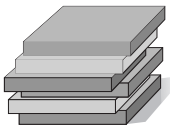
\includegraphics[height=3cm]{Imágenes/prototipo1.png}
    \caption{\textit{Prototipo de Parches}}
    \label{exemploLabel}
    \end{figure}
    
\subsubsection{Prototipo no Operacional }
La segunda concepción de prototipo es la del modelo a escala no funcional, empleado para probar ciertos aspectos del diseño. Un ejemplo es el modelo a escala completa de un automóvil que se utiliza en pruebas de túnel de viento. El tamaño y la forma del automóvil son precisos, pero el automóvil no es funcional; se incluyen sólo las características esenciales para una prueba específica.

Los usuarios de todas formas podrían tomar decisiones en cuanto a la utilidad del sistema con base en el prototipo de la entrada y la salida.

\begin{figure}[h!]
    \centering
    %Modificando los parámetros de height puedes cambiar el tamaño de tu imagen.
    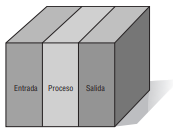
\includegraphics[height=3cm]{Imágenes/prototipo2.png}
    \caption{\textit{Prototipo no Operacional}}
    \label{exemploLabel}
    \end{figure}
    
\subsubsection{Prototipo Primero de un Serie}
La tercera concepción de los prototipos es la creación de un modelo a escala completa de un sistema, a lo que comúnmente se le conoce como piloto. Un ejemplo sería crear el prototipo del primer aeroplano de una serie y después ver si puede volar antes de construir un segundo aeroplano. El prototipo es completamente funcional; es una realización de lo que el diseñador espera sea una serie de aeroplanos con características idénticas. Este tipo de prototipo es útil cuando se planean muchas instalaciones del mismo sistema de información. El modelo funcional a escala completa permite a los usuarios experimentar una interacción realista con el nuevo sistema, al tiempo que minimiza el costo de solucionar los problemas que presenta. Por ejemplo, cuando una cadena de tiendas de abarrotes al menudeo intenta usar el intercambio electrónico de datos (EDI) para verificar los envíos de los proveedores en varios puntos de venta, se podría instalar un modelo a escala completa en una tienda.

\begin{figure}[h!]
    \centering
    %Modificando los parámetros de height puedes cambiar el tamaño de tu imagen.
    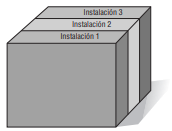
\includegraphics[height=3cm]{Imágenes/prototipo3.png}
    \caption{\textit{Prototipo Primero de un Serie}}
    \label{exemploLabel}
    \end{figure}
    
\subsubsection{Prototipo De Características Selectas }
La cuarta concepción de los prototipos es la creación de un modelo operacional que incluya sólo algunas características del sistema final. Una analogía sería un nuevo centro comercial que abra antes de terminar de construir todas las tiendas. Al crear prototipos de sistemas de información de esta forma, es posible incluir sólo algunas características esenciales. Por ejemplo, el prototipo de un sistema mostraría a los usuarios un menú de pantalla con seis características, agregar un registro, actualizar un registro, eliminar un registro, buscar una palabra clave en un registro, listar un registro o escanear un registro, aunque sólo tres de las seis características estarían habilitadas para usarse, de manera que el usuario pueda agregar un registro (característica 1), eliminar un registro (característica 3) y listar un registro (característica 5). La retroalimentación de los usuarios puede ayudar a los analistas a comprender lo que funciona y lo que no. También puede ayudar con las sugerencias sobre cuáles pueden ser las siguientes características a agregar.

\begin{figure}[h!]
    \centering
    %Modificando los parámetros de height puedes cambiar el tamaño de tu imagen.
    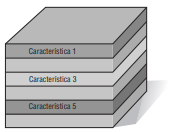
\includegraphics[height=3cm]{Imágenes/prototipo4.png}
    \caption{\textit{Prototipo De Características Selectas}}
    \label{exemploLabel}
    \end{figure}
    
    
\subsection{Uso de prototipos como alternativa para el SDLC }
Algunos analistas argumentan que es necesario considerar a los prototipos como una alternativa al SDLC. En el capítulo 1 vimos que el SDLC es una metodología lógica y sistemática para desarrollar sistemas de información. Las quejas sobre tener que pasar por el proceso del SDLC se concentran en dos aspectos interrelacionados. El primero es el largo tiempo requerido para pasar por el ciclo de vida de desarrollo. A medida que aumenta la inversión de tiempo del analista, el costo del sistema entregado se eleva en forma proporcional. La segunda es que los requerimientos del usuario cambian con el tiempo. Durante el extenso intervalo entre el momento en que se analizan los requerimientos de los usuarios y el momento en el que se entrega el sistema terminado, los requerimientos de los usuarios evolucionan. Así, debido al ciclo de desarrollo extendido, puede suceder que el sistema resultante reciba críticas por abordar en forma inadecuada los requerimientos de información actuales de los usuarios.



\section{Desarrollo de un Prototipo}
Los prototipos son un medio excelente para obtener retroalimentación sobre el sistema propuesto y el grado en que cumple con las necesidades de información de sus usuarios, como se muestra en la figura 6.2. El primer paso de la creación de un prototipo es estimar los costos involucrados en la construcción de un módulo del sistema. Si los costos del tiempo de los programadores y del analista, así como los costos del equipo están dentro del presupuesto, se puede continuar con la construcción del prototipo. Ésta es una excelente manera de facilitar la integración del sistema de información en la cultura y sistema, más extensos, de la organización.

\begin{figure}[h!]
    \centering
    %Modificando los parámetros de height puedes cambiar el tamaño de tu imagen.
    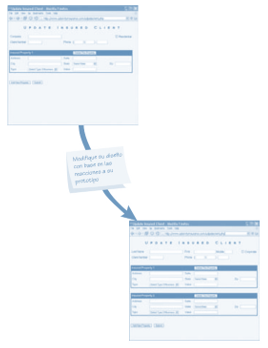
\includegraphics[height=12cm]{Imágenes/desarollo-prototipo.png}
    \caption{\textit{Desarrollo de Prototipos}}
    \label{exemploLabel}
    \end{figure}
\subsection{Lineamientos para desarrollar un Prototipo}
Una vez tomada la decisión de crear un prototipo, hay que cumplir con cuatro lineamientos para integrar el prototipo en la fase de determinación de requerimientos del SDLC: 
\begin{enumerate}
\item Trabajar en módulos administrables. 
\item Crear el prototipo con rapidez. 
\item Modificar el prototipo.
\item Hacer énfasis en la interfaz de usuario. 
\end{enumerate}

\subsubsection{Trabajar En Módulos Administrables }
Un módulo administrable permite a los usuarios interactuar con sus características clave y se puede construir por separado. Las características del módulo que se consideran menos importantes se dejan intencionalmente fuera del prototipo inicial. Como veremos más adelante en este capítulo, esto es muy similar a la metodología ágil que hace énfasis en liberar pequeñas versiones. 

\subsubsection{Crear El Prototipo Con Rapidez }
Los analistas pueden usar prototipos para acortar este hueco mediante el uso de técnicas tradicionales de recopilación de información para señalar los requerimientos salientes de información, y después tomar decisiones rápidas que produzcan un modelo funcional. En efecto, el usuario ve y utiliza el sistema desde las primeras etapas del SDLC, en vez de tener que esperar un sistema terminado para obtener experiencia práctica.
    
\subsubsection{Modificar El Prototipo }
Por lo general el prototipo se modifica varias veces, para lo cual pasa a través de varias iteraciones. Los cambios en el prototipo deben acercar más el sistema a lo que los usuarios dicen que es importante. Cada modificación requiere de otra evaluación por parte de los usuarios. El prototipo no es un sistema terminado. Entrar a la fase de creación del prototipo con la idea de que requerirá modificaciones es una postura útil que demuestra a los usuarios qué tan necesaria es su retroalimentación para mejorar el sistema. 

\subsubsection{Hacer Énfasis En La Interfaz De Usuario }
La interfaz del usuario con el prototipo (y con el sistema, en última instancia) es muy importante. Como lo que realmente tratamos de lograr con el prototipo es hacer que los usuarios articulen con más detalle sus requerimientos de información, deben ser capaces de interactuar con facilidad con el prototipo del sistema. También deben ser capaces de ver cómo el prototipo les permitirá realizar sus tareas. Para muchos usuarios, la interfaz es el sistema. No debe ser un obstáculo.

\subsection{Desventajas de los Prototipos }
Al igual que sucede con cualquier otra técnica de recopilación de información, el uso de prototipos presenta varias desventajas. 
La primera es que puede ser bastante difícil administrar la creación de un prototipo como un proyecto dentro del esfuerzo más grande de sistemas.
La segunda es que los usuarios y analistas pueden adoptar un prototipo como sistema completo cuando todavía es inadecuado y aunque nunca haya tenido la intención de servir como sistema terminado. 

\subsection{Ventajas de los Prototipos }
La utilización de prototipos no es necesaria o apropiada en todos los proyectos de sistemas, como hemos visto. Sin embargo, las ventajas también se deben tener en consideración al decidir si debemos o no crearlos. Las tres principales ventajas de los prototipos son el potencial de cambiar el sistema durante las primeras etapas de su desarrollo, la oportunidad de detener el desarrollo en un sistema que no está funcionando y la posibilidad de desarrollar un sistema que cumpla mejor con las necesidades y expectativas de los usuarios. 

\subsection{Creación de prototipos mediante software COTS }
Algunas veces, la forma más rápida de crear un prototipo es por medio de la instalación modular de software COTS. Aunque podemos explicar con facilidad el concepto de COTS a través de los populares paquetes de un costo relativamente bajo tales como los productos Microsoft Office, hay otros paquetes de software COTS elaborados y costosos, pero muy útiles. 

\subsection{El papel que desempeñan los usuarios en los prototipos }
Sin la participación de los usuarios, los prototipos no tienen mucho sentido. Los comportamientos precisos necesarios para interactuar con un prototipo pueden variar, pero está claro que el usuario es fundamental para el proceso de creación de prototipos. Teniendo en cuenta la importancia del usuario para el éxito del proceso, los miembros del equipo de análisis de sistemas deben fomentar y agradecer la entrada y protegerse contra su propia resistencia natural a cambiar el prototipo. Hay tres formas principales en las que un usuario puede ayudar con los prototipos: 
\begin{enumerate}
\item Experimentar con el prototipo. 
\item Ofrecer reacciones abiertas al prototipo. 
\item Sugerir lo que se puede agregar o quitar en el prototipo.
\end{enumerate}
\begin{figure}[h!]
    \centering
    %Modificando los parámetros de height puedes cambiar el tamaño de tu imagen.
    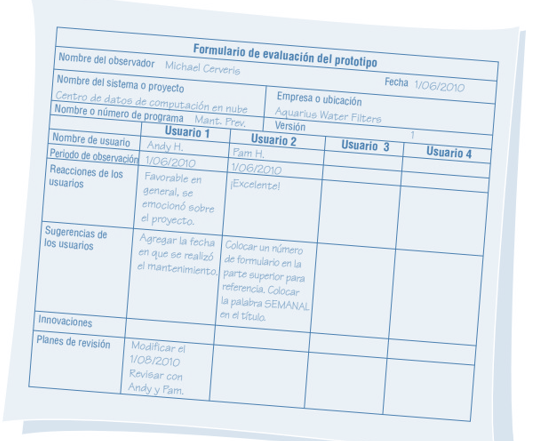
\includegraphics[height=10cm]{Imágenes/formulacion-prototipo.png}
    \caption{\textit{Desarrollo de Prototipos}}
    \label{exemploLabel}
    \end{figure}
\section{Modelado Ágil}
Los métodos ágiles son una colección de metodologías innovadoras para el desarrollo de sistemas, las cuales se centran en los usuarios.A estos métodos se les acreditan muchos proyectos exitosos de desarrollo de sistemas y en muchos casos también se les acredita el haber rescatado empresas de un sistema fallido diseñado mediante el uso de una metodología estructurada.

\subsection{Los Principios Básicos Del Modelado Ágil  }
Los principios ágiles son reflejos y especificaciones de los valores ágiles. Sirven como lineamientos que los desarrolladores pueden seguir al desarrollar sistemas. También sirve para diferenciar a las metodologías ágiles de las metodologías más tradicionales basadas en planes como SDL, así como las metodologías orientadas a objetos. Beck y sus colaboradores fueron los primeros en describir los principios ágiles, que han evolucionado desde entonces. Estos principios se pueden expresar en una serie de dichos tales como: 
\begin{enumerate}
\item Satisfacer al cliente por medio de la entrega de software funcional. 
\item Adoptar el cambio, incluso si se introduce en las últimas etapas del desarrollo. 
\item Seguir entregando software funcional en incrementos y con frecuencia. 
\item Fomentar a los clientes y analistas a que trabajen juntos a diario. 
\item Confiar en los individuos motivados para que realicen su trabajo. 
\item Promover la conversación cara a cara. 
\item Concentrarse en hacer que el software funcione.
\item Fomentar el desarrollo continuo, regular y sostenible.
\item Confiar en los individuos motivados para que realicen su trabajo. 
\item Promover la conversación cara a cara. 
\item Concentrarse en hacer que el software funcione.
\item Fomentar el desarrollo continuo, regular y sostenible.
\item Adoptar la agilidad con especial atención en un diseño lúcido.
\item Apoyar a los equipos autoorganizados. 
\item Proveer retroalimentación rápida. 
\item Fomentar la calidad. 
\item Revisar y ajustar el comportamiento de vez en cuando. 
\item Adoptar la simpleza.
\end{enumerate}

\subsection{Actividades, recursos y prácticas del modelado ágil }
El modelado ágil involucra una serie de actividades a completar en cierto momento durante el proceso de desarrollo ágil. En esta sección hablaremos sobre esas actividades, los recursos y las prácticas que son únicas para la metodología ágil. 

\subsubsection{Cuatro Actividades Básicas Del Desarrollo Ágil }
Hay cuatro actividades básicas de desarrollo que utilizan los métodos ágiles: codificar, probar, escuchar y diseñar. El analista necesita identificar el grado de esfuerzo requerido por cada actividad para compararlo con los recursos necesarios para completar el proyecto. La codificación es la actividad indispensable. El proceso es fundamentalmente el siguiente: elija una idea, codifíquela, pruébela y compruebe si la idea era lógica. El código también se puede usar para comunicar ideas que, de otra manera, permanecerían borrosas o deformes; cuando examine su código, tal vez incluso le surjan nuevas ideas. El código fuente es la base de un sistema viviente. Es esencial para el desarrollo.
\begin{enumerate}
\item TIEMPO.    Hay que asignar tiempo suficiente para completar el sistema, y entender que lo necesita para varias actividades distintas: escuchar a los clientes, diseñar, codificar y probar. 
\item COSTO.    Suponga que las actividades de codificación, diseño, prueba y escucha están sobrecargando el proyecto y los recursos que invertimos en el tiempo, alcance y la calidad no son suficientes, incluso aunque dediquemos una cantidad normal al costo para equilibrar el proyecto. 
\item CALIDAD.  La importancia de la calidad y los métodos (como TQM y Seis Sigma) que ayudan a asegurar un alto grado de calidad en el software.
\item ALCANCE.  Para determinar el alcance hay que escuchar a los clientes y hacer que escriban sus historias, que se examinan después para determinar cuánto se puede hacer en un tiempo dado para satisfacerlos.
\end{enumerate}

\subsubsection{Cuatro Practicas Agiles  Básicas }
\begin{enumerate}
\item En las entregas pequeñas, el equipo de desarrollo comprime el tiempo entre entregas de su producto. Envez de entregar una versión completa con todas las características en un año, mediante el uso de la práctica de entregas pequeñas reducen el tiempo de entrega al resolver las características más importantes primero y entregar ese sistema o producto para mejorarlo más adelante.
\item Esta práctica básica intenta motivar a los miembros del equipo para que trabajen en forma intensa y después se tomen tiempo de descanso, para que cuando regresen se encuentren relajados y menos estresados. Esto ayuda a los miembros del equipo a detectar problemas con más facilidad, al tiempo que evita costosos errores y omisiones debido a un rendimiento inefectivo o al agotamiento.
\item Alojar al cliente en el sitio; es decir, tener “en casa”, durante el proceso de desarrollo, a un usuario experto en el aspecto de negocios relacionado con el trabajo de desarrollo de sistemas. Esta persona es muy importante para el proceso: escribe las historias de los usuarios, se comunica con los miembros del equipo, ayuda a asignar prioridades y equilibrar las necesidades a largo plazo de la empresa, y toma decisiones en cuanto a la característica que se deba resolver primero.
\item La programación en pareja es una importante práctica básica. Aquí usted trabaja con otro programador que usted mismo haya elegido. Ambos realizan la codificación y las pruebas. A menudo la persona con más experiencia emprenderá el proceso de codificación primero, pero a medida que la menos experimentada se empiece a involucrar, el que tenga la visión clara sobre el objetivo será quien se encargue de la codificación.
\end{enumerate}

\subsection{El proceso de Desarrollo Agil}
El modelado es una palabra clave en los métodos ágiles. El modelado ágil aprovecha la oportunidad de crear modelos que pueden ser lógicos, como los dibujos de los sistemas, o maquetas de tamaño natural como los prototipos que describimos anteriormente en este capítulo. Un proceso ordinario de modelado ágil podría ser el  siguiente:
\begin{enumerate}
\item Escuchar las historias de los usuarios por medio del cliente.
\item Dibujar un modelo del flujo de trabajo lógico para apreciar las decisiones de negocios representadas en la historia de un usuario.
\item Crear historias de usuarios con base en el modelo lógico.
\item Desarrollar algunos prototipos de visualización. Para ello hay que mostrar a los clientes el tipo de interfaz que tendrán. 
\item Usar la retroalimentación de los prototipos y los diagramas del flujo de trabajo lógico para desarrollar el sistema hasta crear un modelo físico de datos.
\end{enumerate}

\begin{figure}[h!]
    \centering
    %Modificando los parámetros de height puedes cambiar el tamaño de tu imagen.
    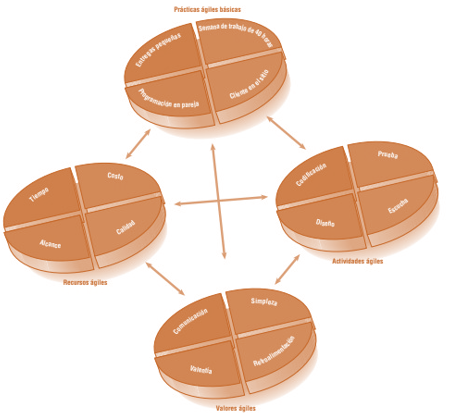
\includegraphics[height=8cm]{Imágenes/Proceso-Agil.png}
    \caption{\textit{Proceso de Desarrollo Agil}}
    \label{exemploLabel}
    \end{figure}
\section{Comparacion entre el Modelado Agil y los Metodos Estructurados}
Es cierto que los proyectos desarrollados por medio de métodos ágiles a menudo requieren de un ajuste para que funcionen de manera apropiada, los desarrolladores ágiles admiten que esto es parte del proceso. La metodología ágil implica muchas entregas pequeñas, y durante el proceso se van agregando más características.
\begin{figure}[h!]
    \centering
    %Modificando los parámetros de height puedes cambiar el tamaño de tu imagen.
    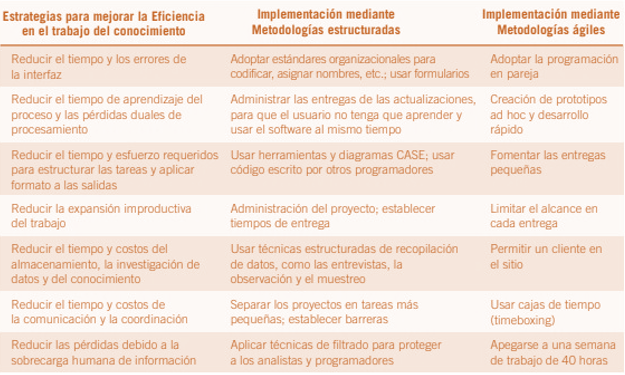
\includegraphics[height=8cm]{Imágenes/tabla-comparacion.png}
    \caption{\textit{Tabla Implementacion de las estrategias de Davis y Naumann para mejorar la eficiencia mediante uso de dos metodologias distintas}}
    \label{exemploLabel}
    \end{figure}
\subsection{Reducción de los tiempos y errores de la interfaz }
Los analistas de sistemas y los programadores necesitan analizar, diseñar y desarrollar sistemas mediante el uso de herramientas de trabajo que varían desde Microsoft office hasta herramientas CASE, que son costosas y sofisticadas. También necesitan realizar la documentación a medida que desarrollan sistemas. Es importante que los analistas y los programadores sean capaces de comprender la interfaz que utilizan. Necesitan saber cómo clasificar, codificar, almacenar y escribir sobre los datos que recopilan. Los desarrolladores de sistemas también necesitan acceder con rapidez a un programa, escribir la información requerida y recuperarla cuando la necesiten de nuevo.

\subsection{Reducir el tiempo de aprendizaje del proceso y las pérdidas duales de procesamiento }
Los analistas y los programadores aprenden técnicas específicas y lenguajes de software requeridos para completar un proyecto actual. A menudo se producen ineficiencias cuando algunos analistas y programadores ya conocen los productos que se van a utilizar, mientras que otros aún necesitan aprender a usarlos. Por lo general pedimos que los desarrolladores aprendan a usar estos productos al mismo tiempo que los utilizan para construir el sistema. Esta capacitación en el trabajo ralentiza de manera considerable el proyecto de desarrollo de sistemas en su totalidad. Un proyecto tradicional y estructurado requiere más aprendizaje.

\subsection{Reducción del tiempo y esfuerzo requeridos para estructurar tareas y aplicar formato a las salidas  }
Cada vez que un proyecto se inicia, los desarrolladores necesitan determinar los límites. En otras palabras, necesitan saber cuál será el producto entregable y cómo organizarán el proyecto de manera que puedan completar todas las tareas necesarias. Una metodología tradicional incluiría el uso de herramientas CASE, dibujar diagramas (como los diagramas E-R y los de flujo de datos), usar software de administración de proyectos (como Microsoft Project), descripciones de trabajo muy detalladas, usar y reutilizar formularios y plantillas, y reutilizar el código escrito por otros programadores. 

\subsection{Reducción de la expansión improductiva del trabajo }
La ley de Parkinson establece que “el trabajo se expande para poder llenar el tiempo disponible para completarlo”. Si no hay tiempos de entrega específicos, es posible que el trabajo del conocimiento continúe su expansión. Con las metodologías estructuradas tradicionales, al principio los tiempos de entrega parecen estar muy alejados hacia el futuro. Los analistas pueden utilizar técnicas de administración de proyectos para tratar de programar las actividades, pero hay una predisposición integrada en cuanto a extender las primeras tareas más de lo necesario y después tratar de acortarlas en una etapa posterior del desarrollo. Los analistas y los programadores se preocupan menos por los tiempos de entrega distantes que por los que ya están próximos. 

\subsection{Reducción del tiempo y costos de almacenamiento y de la investigación de los datos y del conocimiento }
Los desarrolladores de sistemas necesitan recopilar información sobre la organización, los objetivos, las prioridades y los detalles acerca de los sistemas de información actuales antes de proceder con el desarrollo de un nuevo sistema.

\subsection{Reducción de los tiempos y costos de la comunicación y la coordinación }
La comunicación entre analistas y usuarios, así como entre los mismos analistas, es la base del desarrollo de sistemas. Sin duda una mala comunicación es la raíz de múltiples problemas de desarrollo. Sabemos que la comunicación aumenta cuando se unen más personas al proyecto. 

\subsection{Reducción de las pérdidas debido a la sobrecarga humana de información }
Una situación de sobrecarga parecida le puede ocurrir a cualquier persona en cualquier momento, incluyendo a los analistas de sistemas y a los programadores. Una metodología tradicional sería tratar de filtrar información para proteger a los analistas y programadores de las quejas de los clientes. Esta metodología permite a los desarrolladores seguir trabajando en el problema sin la interferencia y subjetividad que existirían en una situación normal. Mediante el uso de una filosofía ágil, los analistas y programadores se deben apegar a una semana de trabajo de 40 horas. 
    
\subsection{Riesgos inherentes a la innovación organizacional }
Al consultar con los usuarios, los analistas deben considerar los riesgos a los que se enfrentan las organizaciones al adoptar nuevas metodologías. Sin duda esto está relacionado con el momento apropiado para actualizar las habilidades humanas, adoptar nuevos procesos organizacionales e instituir el cambio interno. En un sentido más amplio, éstas son preguntas de dimensión estratégica para el liderazgo organizacional. Consideremos de manera específica el caso del equipo de análisis de sistemas que adopta los métodos ágiles en virtud de los riesgos para la organización y el resultado exitoso eventual para el equipo de desarrollo de sistemas y sus clientes.
    
\begin{figure}[h!]
    \centering
    %Modificando los parámetros de height puedes cambiar el tamaño de tu imagen.
    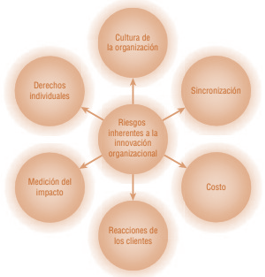
\includegraphics[height=8cm]{Imágenes/riesgos.png}
    \caption{\textit{Variables para evaluar el riesgo de adoptar una innovacion organizacional}}
    \label{exemploLabel}
    \end{figure}  
    
    \\
CULTURA DE LA ORGANIZACION \par
Una cultura organizacional conservadora con muchas características estables que no busque innovar puede ser un contexto inapropiado, e incluso inhóspito, para que el grupo de desarrollo de sistemas adopte las metodologías ágiles.\par
SINCRONIZACION\par
Las organizaciones deben hacer y responder la pregunta acerca de cuándo es el mejor momento para innovar con la adopción de nuevas metodologías de desarrollo de sistemas, cuando se tienen en cuenta todos los proyectos y factores (internos y externos). Las organizaciones deben tener en cuenta toda la variedad de proyectos en los que están invirtiendo, mirar más allá de los tiempos de entrega de los proyectos, programar la actualización de las plantas físicas y absorber las proyecciones clave en la industria y la economía.\par
COSTO\par
Otro de los riesgos en cuanto a la adopción de metodologías ágiles para las organizaciones es el costo involucrado en la educación y capacitación de los analistas de sistemas y programadores en relación con la nueva metodología. Esto puede implicar costos de seminarios y cursos fuera del sitio de trabajo, o tal vez haya que contratar consultores para que trabajen con el personal actual en el sitio.\par
REACCIONES DE LOS CLIENTES\par
Cuando los clientes (ya sean internos o externos) se involucran como usuarios o iniciadores de los esfuerzos de desarrollo de sistemas de información, las reacciones en cuanto al uso de nuevos métodos requeridos por la metodología ágil también son una consideración clave. Algunos clientes reaccionan de manera alegre una vez que se les describen los beneficios de la conveniencia en tiempo y la participación.\par
MEDICION DEL IMPACTO\par
Otra consideración para las organizaciones que adoptan metodologías ágiles es cómo certificar y medir que los nuevos métodos van a facilitar el desarrollo exitoso de sistemas. Las fortalezas y debilidades de los métodos estructurados tradicionales que se utilizan para desarrollar sistemas de información son muy conocidas. Aunque hay mucha evidencia anecdótica para establecer que las metodologías ágiles son superiores para el desarrollo bajo ciertas condiciones, su historial es corto y aún no se cuenta con soporte empírico.\par
LOS DERECHOS INDIVIDUALES DE LOS PROGRAMADORES-ANALISTAS\par
Los desarrolladores (analistas y programadores) de sistemas exitosos ejercen creatividad en cuanto a la forma de llevar a cabo su trabajo, por lo cual merecen el derecho de trabajar en la configuración más fructífera posible. Es posible que los requerimientos de trabajo de los nuevos métodos ágiles (por ejemplo, la programación en pareja) vayan en detrimento de ciertos derechos básicos de las personas creativas de trabajar por su cuenta o en grupos.\par



\nocite{*}
\bibliographystyle{apalike}
\bibliography{Libros.bib}

\centering\vspace*{\fill} 
\end{document}

 %Fin del documento.